\documentclass[debug]{beamer} % beamer 3.10: do NOT use option hyperref={pdfpagelabels=false}! 
%\documentclass[final,hyperref={pdfpagelabels=false}]{beamer} % beamer 3.07: get rid of beamer warnings

\mode<presentation>{\usetheme{dsunicamp}}


% Put any other packages or custom macros in here:
\PassOptionsToPackage{main=english}{babel}
\usepackage[english]{babel}
\usepackage[utf8]{inputenc}		% Codificacao do documento (convers\~{a}o autom\'{a}tica dos acentos)
\usepackage[T1]{fontenc}
\usepackage[backend=biber, isbn=false, doi=false,style=ieee,language=english]{biblatex}
\renewcommand*{\bibfont}{\footnotesize}
\setbeamercolor{bibliography item}{parent=palette primary}
\setbeamercolor*{bibliography entry title}{parent=palette primary}
\bibliography{bibliography}


%%%%%%%MATH STUFF
\usepackage{fix-cm}% just to avoid some spurious messages
\usepackage{amsmath}
\usepackage{mathtools}
\usepackage{bm}
\usepackage{exscale} %integral sign in poster
\usepackage{eulervm}
%%%%%%%%%RANDOM STUFF
\usepackage{cleveref} %cref, Cref
\usepackage{microtype} %aligning and stuff
%%%%%%%%%GRAPHICAL STUFF
\usepackage{tikz}
\usepackage{mdframed}
\usepackage{subcaption} %subfigs
\usepackage{graphicx}% http://ctan.org/pkg/graphicx
\usepackage{booktabs}%toprule,midrule,fancy tables in general
\usetikzlibrary{calc}

% Portrait, A0 poster. Set scale as desired, but 1.3 gives easily readable text when printed.
\usefonttheme{metropolis}
\setbeamerfont{block title}{size=\large}
\usepackage[orientation=portrait, size=custom, scale=1.1,width=91.44,height=121.92]{beamerposter}
%\usepackage[orientation=portrait, size=custom, scale=1.1,width=121.92,height=91.44]{beamerposter}
% Set height of page for use in arranging text boxes, after accounting for
% heading, footer etc. This is a bit of a hack, ideally latex should figure
% this out for itself!
% \newlength{\columnheight}
% %133cm is all that remains
% \setlength{\columnheight}{120cm}

\pdfstringdefDisableCommands{%
  \def\\{ }%
  \def\vspace{0.3em}{ }%
}



\newcommand{\hcurl}[1]{H (curl;#1)}
\newcommand{\hzcurl}[1]{H_0(curl;#1)}
\newcommand{\hone}[1]{H^1(#1)}
\newcommand{\hmspace}[1]{H^m(#1)}
\newcommand{\hzone}[1]{H^1_0(#1)}
\newcommand{\testhcurl}[0]{\bm{\varphi}}
\newcommand{\testhone}[0]{\varphi}
\newcommand{\pkspace}[2][k]{\mathbb{P}_{#1}(#2)}
\newcommand{\pkhomospace}[2][k]{\sim{\mathbb{P}}_{#1}(#2)}
\DeclareMathOperator{\curlop}{\nabla \times}
\DeclareMathOperator{\divop}{\nabla \cdot}
\DeclareMathOperator{\gradop}{\nabla}
\DeclareMathOperator{\curlopt}{\nabla_t \times}
\DeclareMathOperator{\divopt}{\nabla_t \cdot}
\DeclareMathOperator{\gradopt}{\nabla_t}

% Define the header information
\title{DEVELOPMENT OF HIGH-ORDER\\ \vspace{0.3em} \texorpdfstring{H(CURL,$\Omega$)}{H(CURL,OMEGA)}-CONFORMING APPROXIMATION SPACES FOR PHOTONIC WAVEGUIDE ANALYSIS}
% \title{Title \\ \vspace{0.3em} second line of title}
\author{Francisco T. Orlandini\texorpdfstring{\textsuperscript{1}}{ }, Hugo E. H. Figueroa\texorpdfstring{\textsuperscript{1}}{ } and Philippe R. B. Devloo\texorpdfstring{\textsuperscript{2}}{ }}
\institute{\texorpdfstring{\textsuperscript{1}}{ }School of Electrical and Computer Engineering, State University of Campinas, Brazil\\
\texorpdfstring{\textsuperscript{2}}{ }School of Civil Engineering, Architecture and Urban Design, State University of Campinas, Brazil}%

% Now start the actual poster
\begin{document}

% Header is automatically generated from the command defined in the theme
% file, the information above and the logos in the logo folder.


% Start of the body:
\begin{frame}
	\vspace{-1em}
    \centering
    \noindent\begin{minipage}[t]{0.45\textwidth}
      \begin{block}{\boxnumber MOTIVATION}
        	\begin{itshape}   % italic abstract
        		High precision approximation of dispersion parameters is a major concern in the design of photonic waveguides and the Computational Electromagnetics(CE) community has sought many different numerical methods in order to achieve this requirement. In the present work, a high-order Finite Element Method(FEM) scheme is introduced as an efficient technique presenting high convergence rates and being able to deal with curved waveguides and lossy inhomogeneous media with transverse anisotropy. The $\hcurl{\Omega}$-conforming elements used in the scheme are a hierarchical construction of the Nédélec elements of the first kind, implemented in the \texttt{NeoPZ} framework. The importance of using non-linear mapped elements when using high-order elements is exposed and real-world scenario results are presented. Finally, the hierarchical construction of the elements is exploited in an example of how \emph{hp}-adaptive finite elements can significantly reduce the number of equations while still achieving high precision results.
        	\end{itshape}
        \end{block}

        \vfill
        \begin{block}{\boxnumber FEM FORMULATION AND THE \texorpdfstring{H(CURL,$\Omega$)}{H(CURL,OMEGA)}-CONFORMING ELEMENTS}
        The formulation used in this work performs modal analysis on the cross-section $\Omega$ of a waveguide for a given angular frequency $\omega$, using $\hcurl{\Omega}$ and $\hone{\Omega}$-conforming elements for the transverse and longitudinal components of the electric field, respectively. It is valid for a domain composed of materials presenting at most transverse-anisotropy. From \textcite{jin14}:

	        Find non-trivial $\left(\beta^2,{e_t}, {e_z}\right) \in (\mathbb{C} \times [\mathbb{C}]^N \times [\mathbb{C}]^M)$ such that:
			\begin{equation}
				\renewcommand{\arraystretch}{1.5}%
	  			 \scalebox{0.9}{% Scale
					$\begin{multlined}\label{eq:fem-hcurl-disc-1}
					    \int_\Omega\left\{\sum_{j}^Ne_{tj}\left[\mu_{zz}^{-1} \left( \nabla_t \times \testhcurl_j \right)\cdot \left( \nabla_t \times \testhcurl_i \right)^*- k_0^2 \bm{\epsilon}_{xy}\testhcurl_j\cdot\testhcurl_i^*\right]\right.\\
					     +\left.\beta^2\sum_{l}^M e_{zk} \left[ \sum_{j}^Ne_{tj} \bm{\mu}_{xy^S}^{-1} \left( \nabla_t \testhone_k +\testhcurl_j \right)\cdot \left(\nabla_t \testhone_k +\testhcurl_i \right)^*-k_0^2\epsilon_{zz} \testhone_k\testhone_k^*\right]\right\}\mathrm{d}\Omega = 0,\\
					     \forall \testhcurl_i \in B_{U_h}\,,\, \testhone_k \in B_{V_h}\text{,}
					\end{multlined}$
				}
			\end{equation}%
			where $B_{U_h}$ and $B_{V_h}$ denote the FEM basis for the finite-dimensional subspaces of $\hcurl{\Omega}$ and $\hone{\Omega}$, respectively.

			The $\hcurl{\Omega}$-conforming elements used in this work are the Nédélec elements of the first kind\parencite{nedelec80} and were constructed in the NeoPZ framework in a hierarchical manner.
        \end{block}

        \vfill
        \begin{block}{\boxnumber EFFECTS OF GEOMETRICAL REPRESENTATION ON CONVERGENCE}
        	In order to benefit from the high-order elements, non-linear mapped elements are essential when dealing with curved geometries. \Cref{fig:convergence-step} compares the convergence rate of the effective index $n_{\text{\emph{eff}}}$ for a step-index optical fiber with polynomial order $k=4$, using three different types of mapped elements.
        	\vspace*{1ex}

        	\begin{figure}[ht]
	            \centering
	            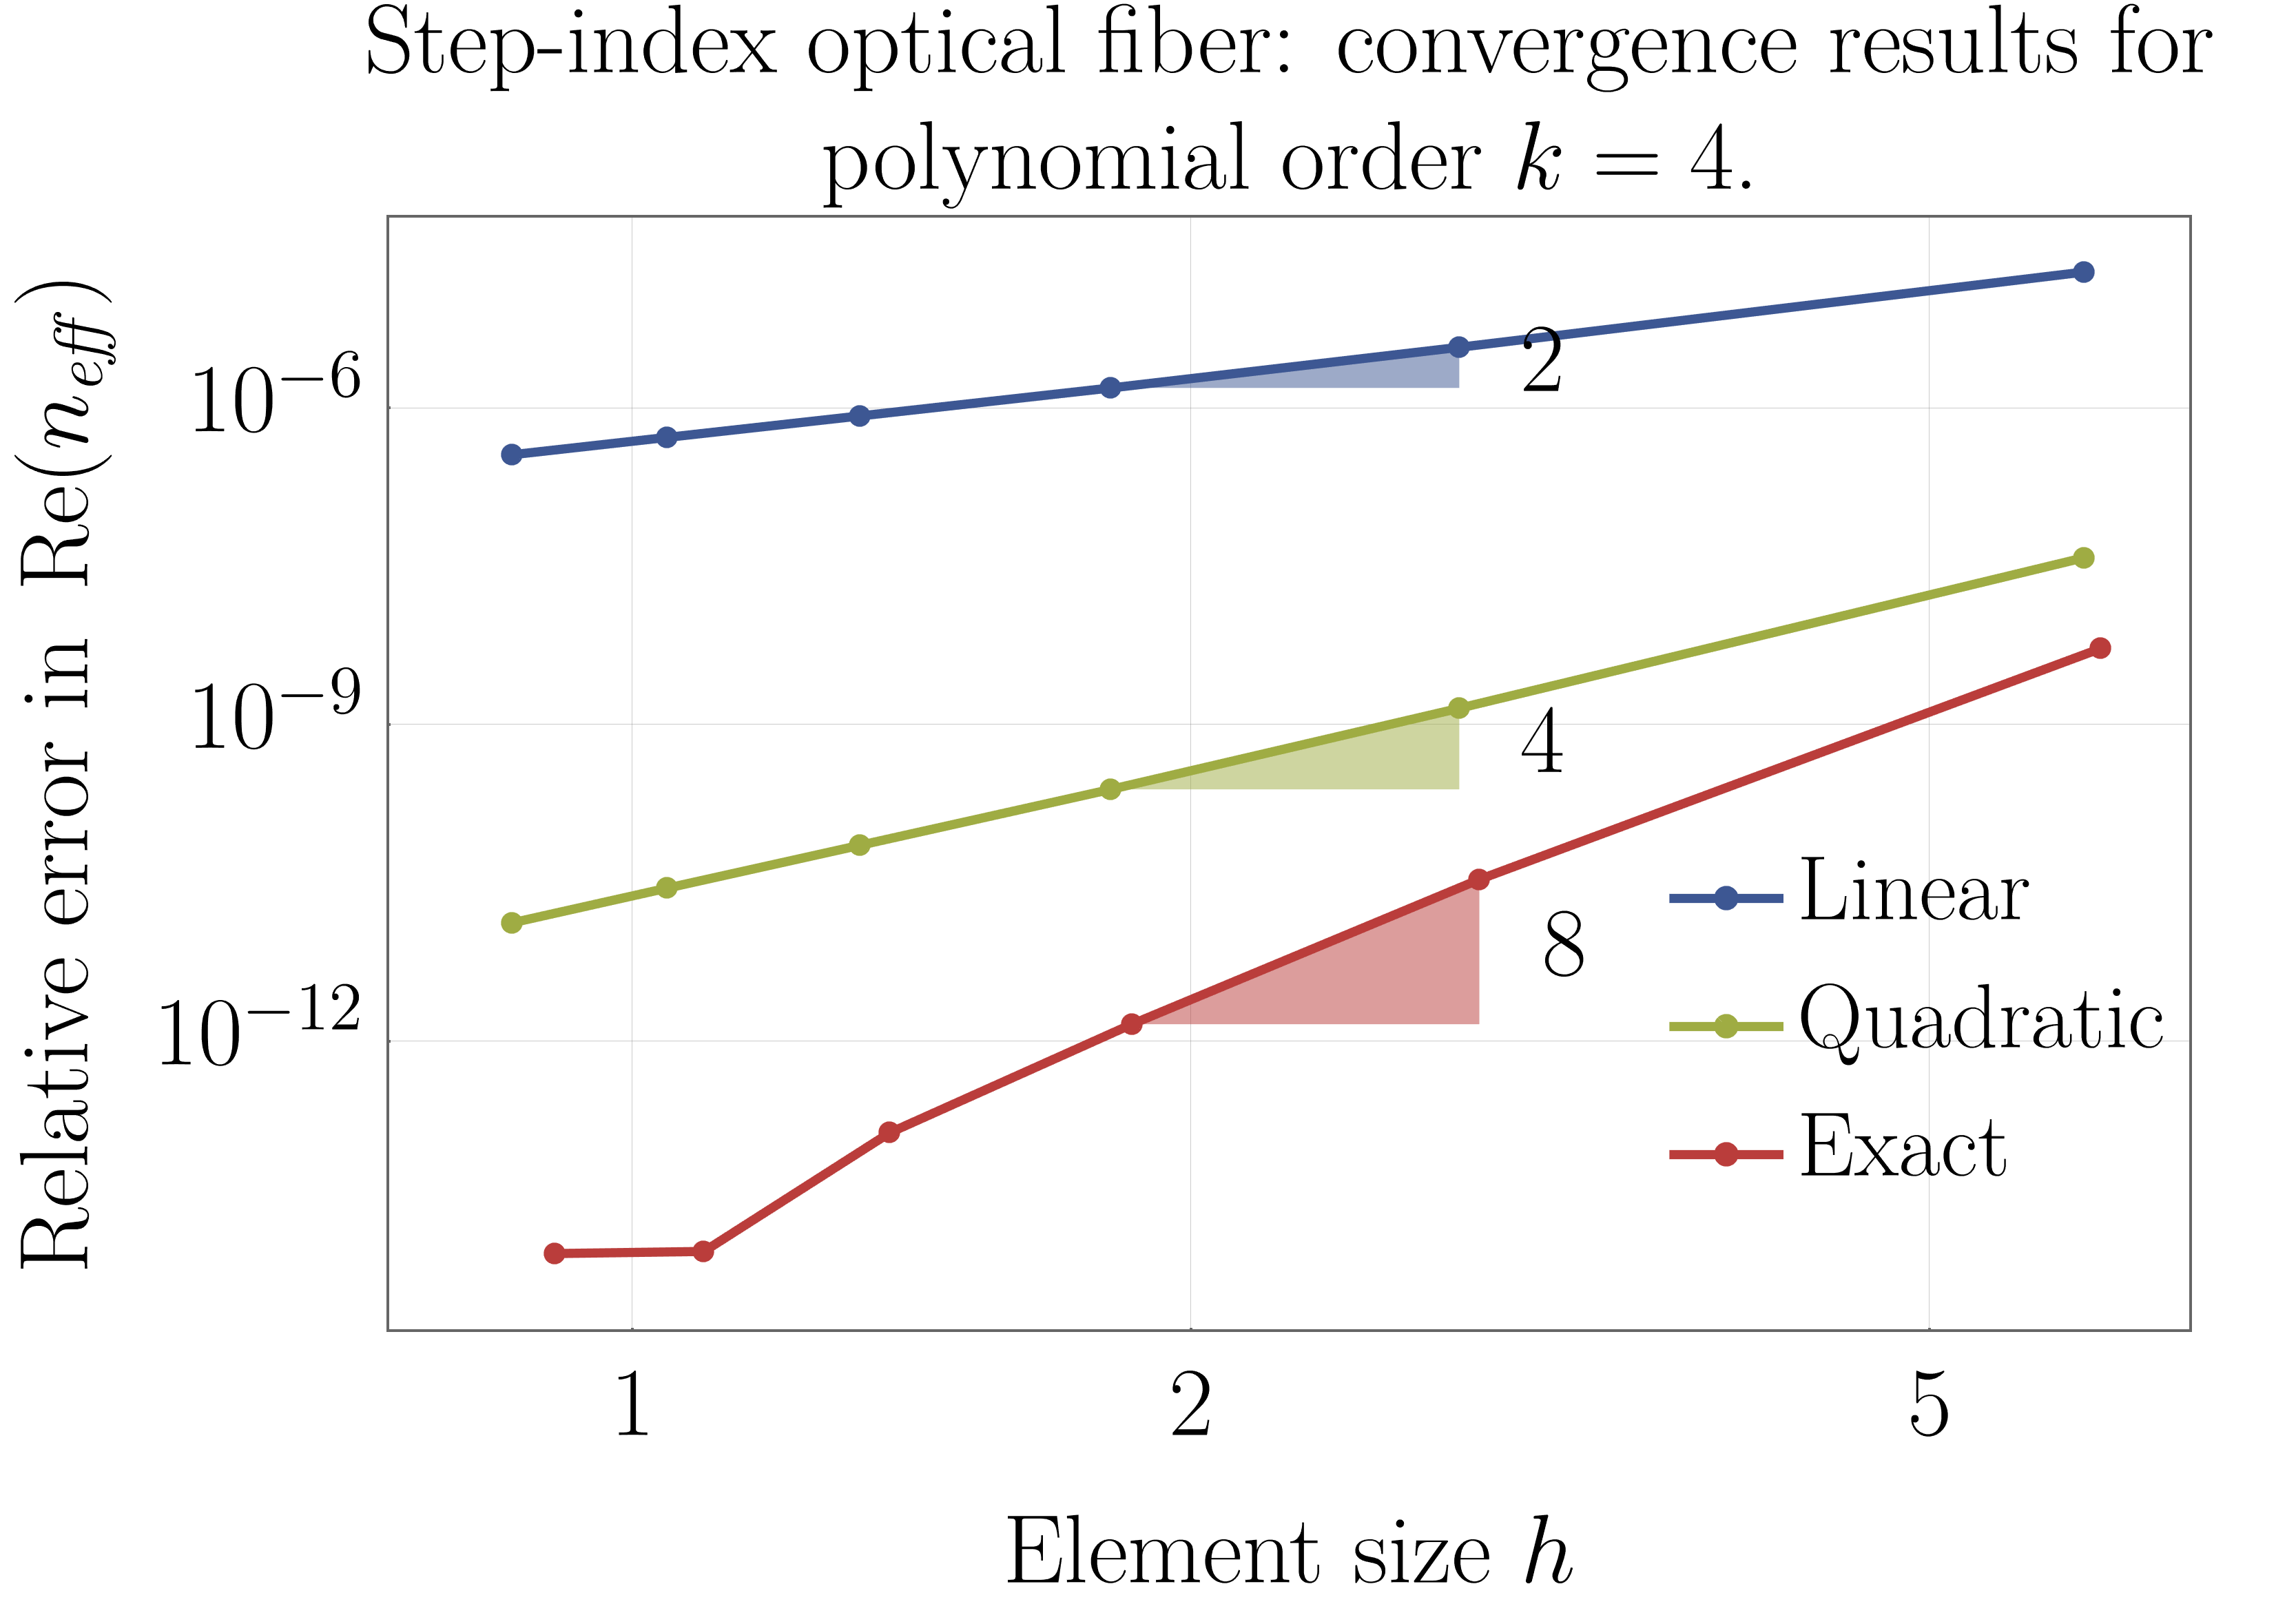
\includegraphics[width=0.7\linewidth]{images/convergenceRates_k4_poster.png}
	            \caption{Comparison of convergence rates for the real part of the effective index of a step-index optical fiber. The polynomial order $k=4$ was used in all three approximations. The geometry was described with elements obtained by linear mapping(blue curve), quadratic mapping(green curve) and exact mapping(red curve).}
	            \label{fig:convergence-step}
        	\end{figure}
        
	        The optimal convergence rate is only obtained with the non-linear mapping: with a fixed number of elements, the linear mapping achieved an error of $10^{-6}$, the quadratic mapping obtained $10^{-11}$, and a relative error of $10^{-13}$ was obtained with the exact mapped elements. \Cref{fig:plot-step} shows two linear polarized modes on the step-index optical fiber.
	        \begin{figure}[hb]
	        	\begin{mdframed}[backgroundcolor=bggrey]
					\centering
					\begin{subfigure}[b]{.4999\textwidth}
						\centering
						\caption*{$\displaystyle\bm{E}_t$}
						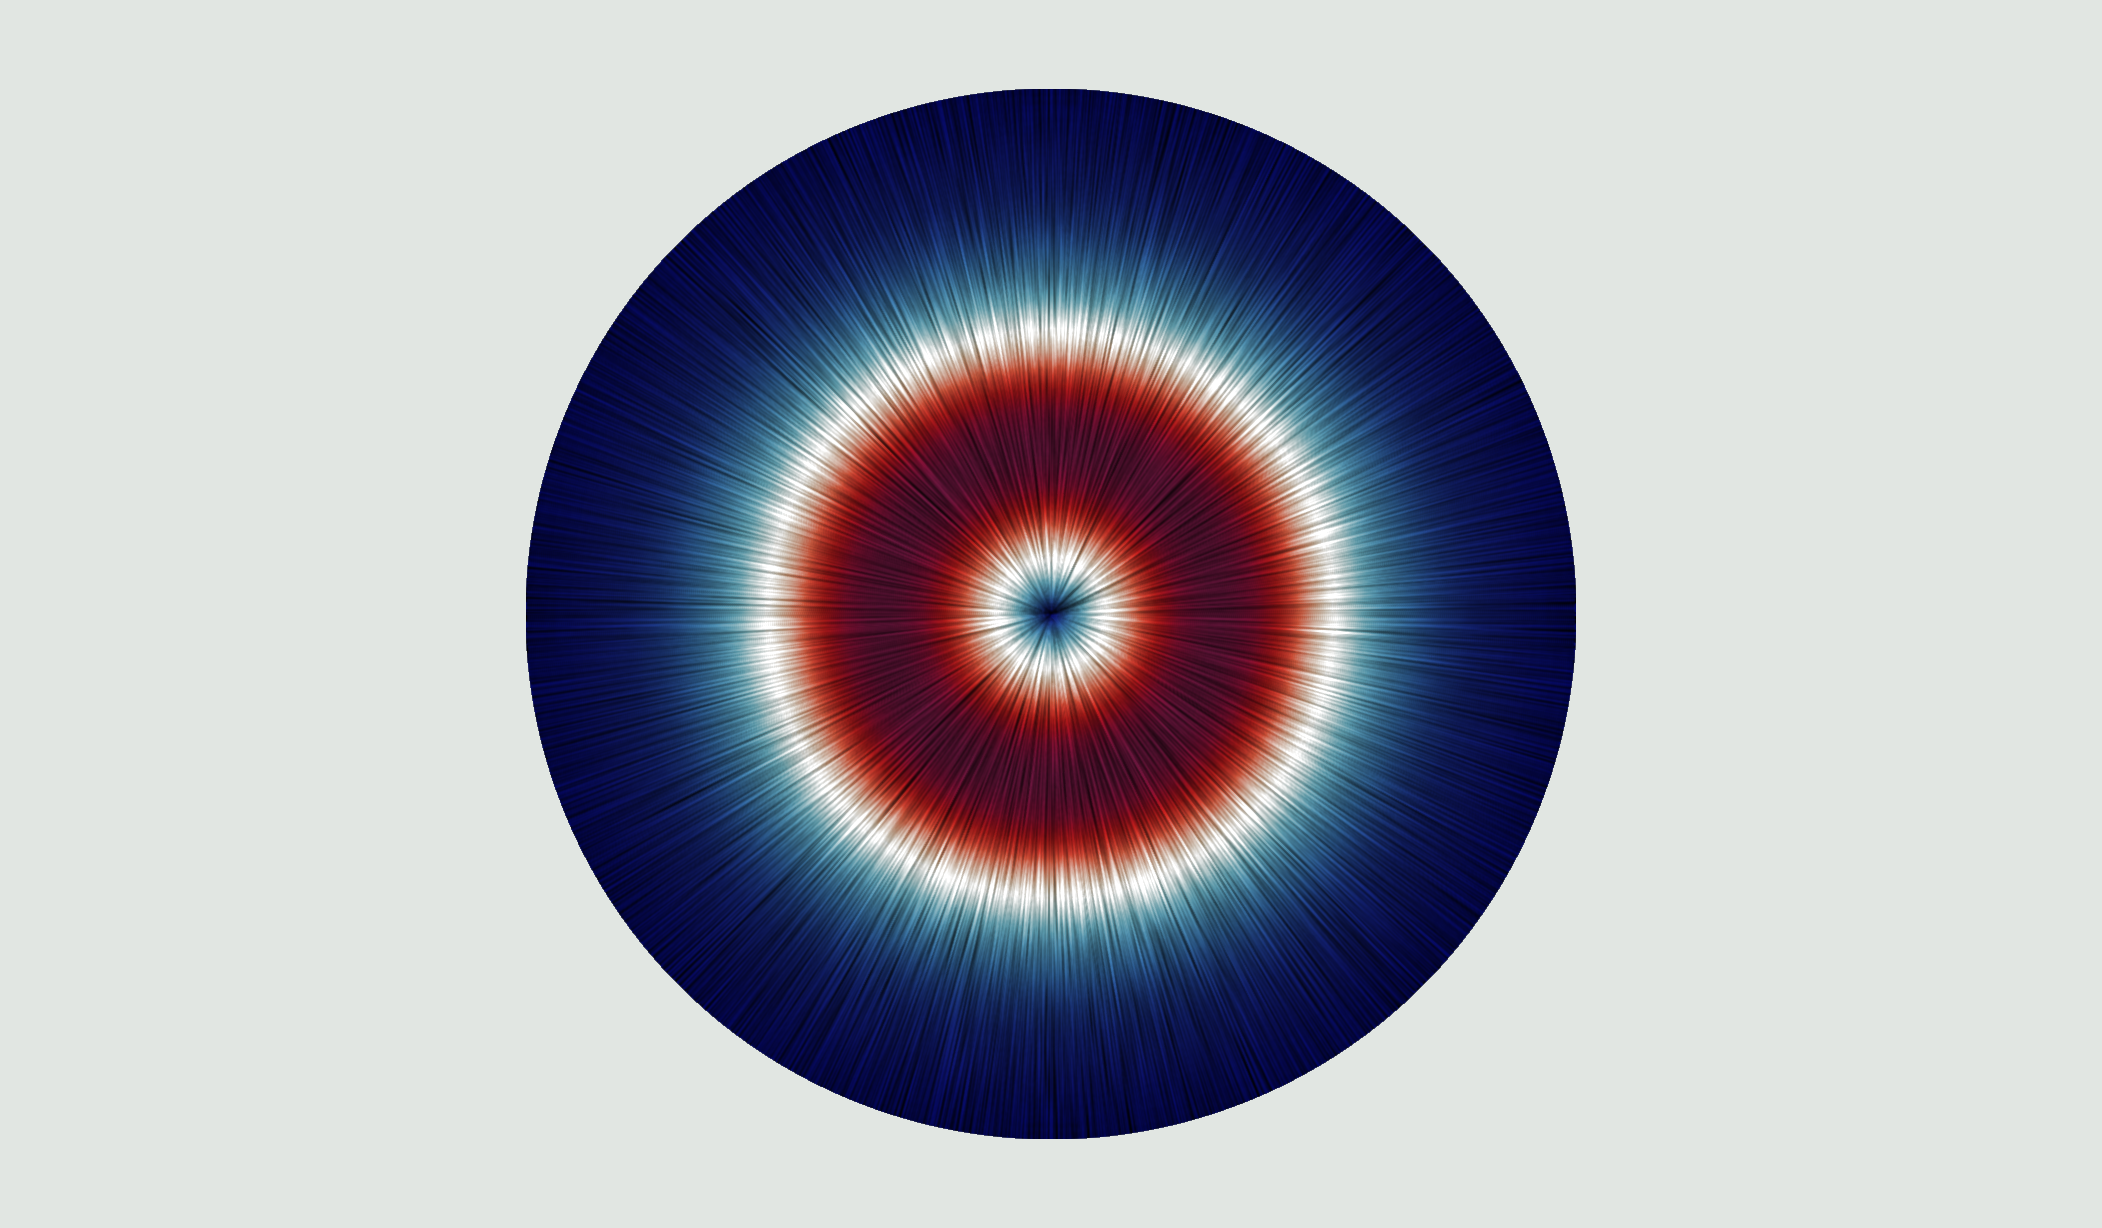
\includegraphics[width=1\linewidth]{images/et2posterStepFiber.png}%
					\end{subfigure}\hfill
					\begin{subfigure}[b]{.4999\textwidth}
						\centering
						\caption*{$\displaystyle E_z$}
						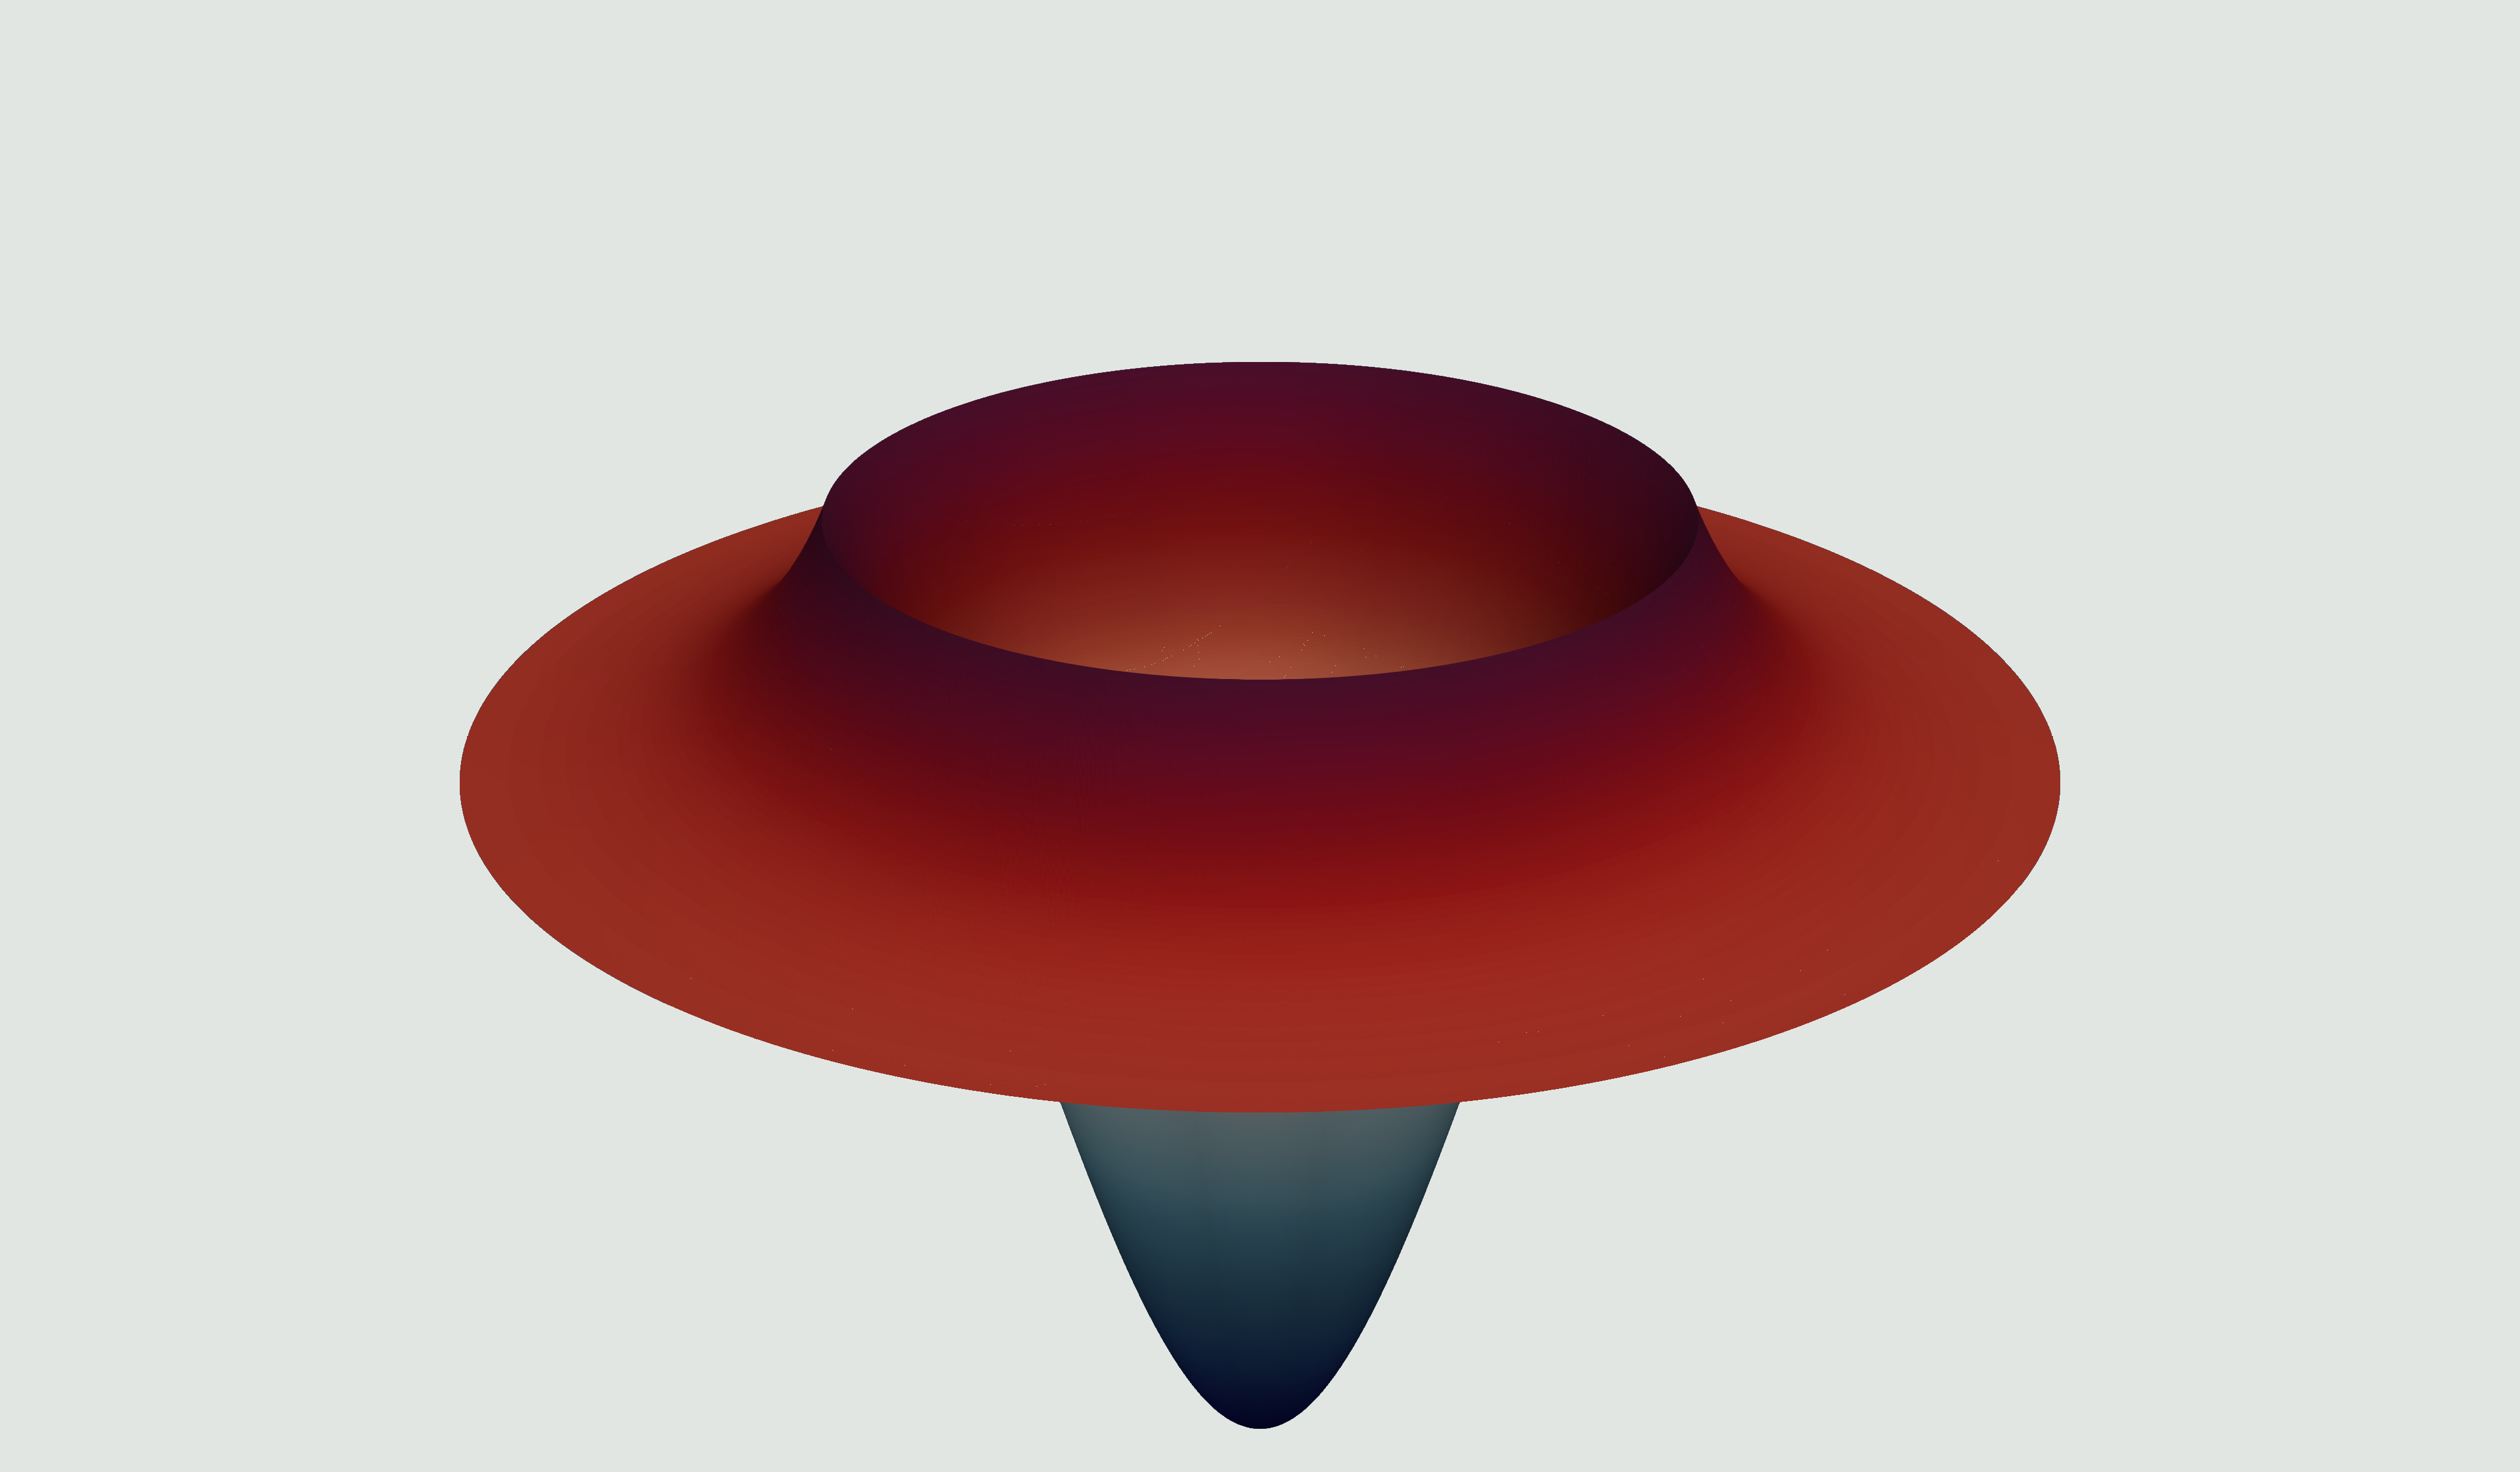
\includegraphics[width=1\linewidth]{images/ez2posterStepFiber.png}%
					\end{subfigure}

					\begin{subfigure}[b]{.4999\textwidth}
						\centering
						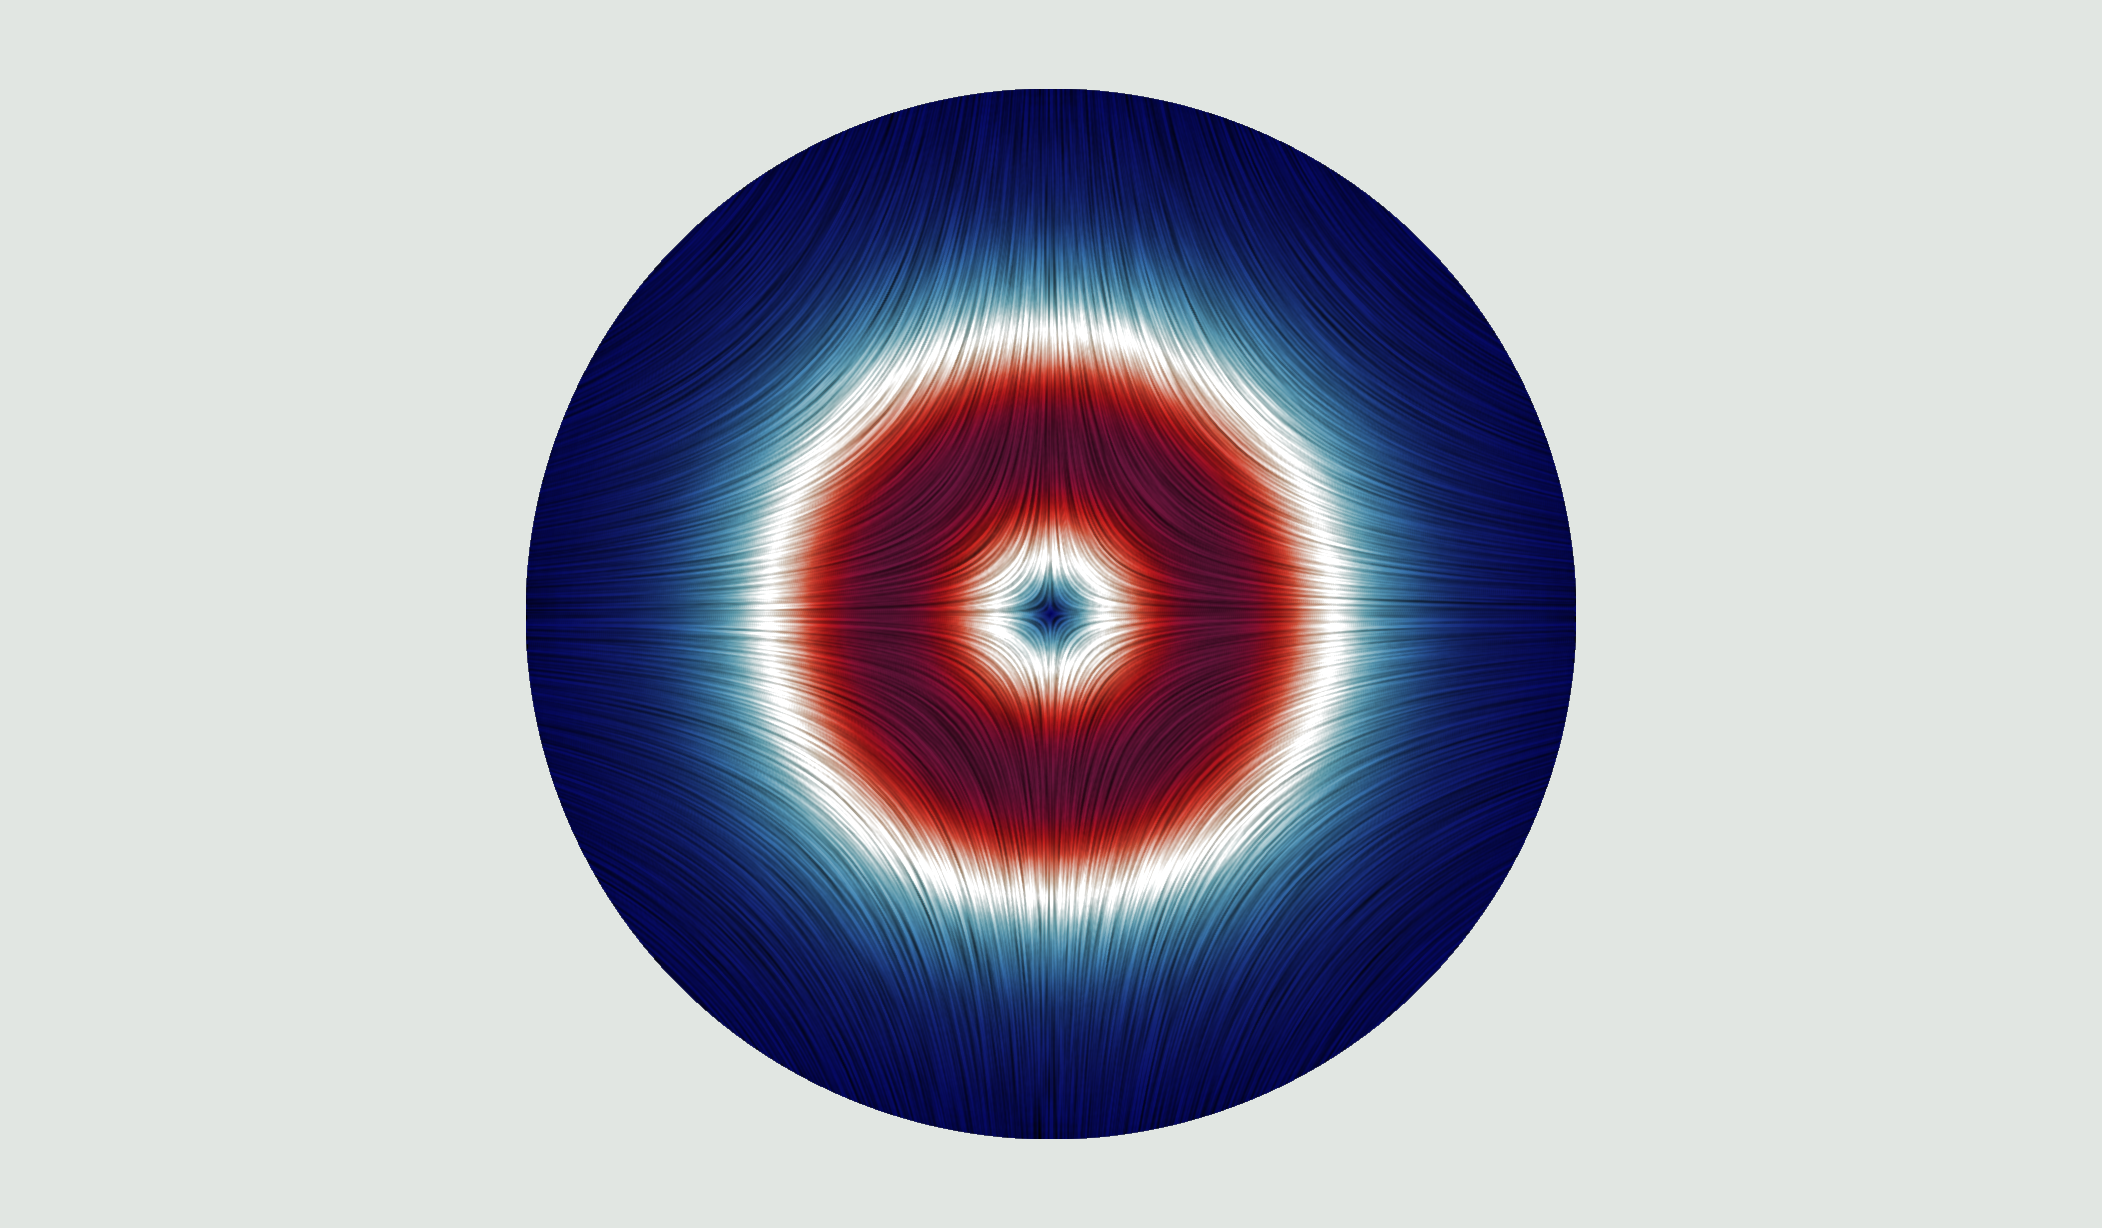
\includegraphics[width=1\linewidth]{images/et3posterStepFiber.png}%
					\end{subfigure}\hfill
					\begin{subfigure}[b]{.4999\textwidth}
						\centering
						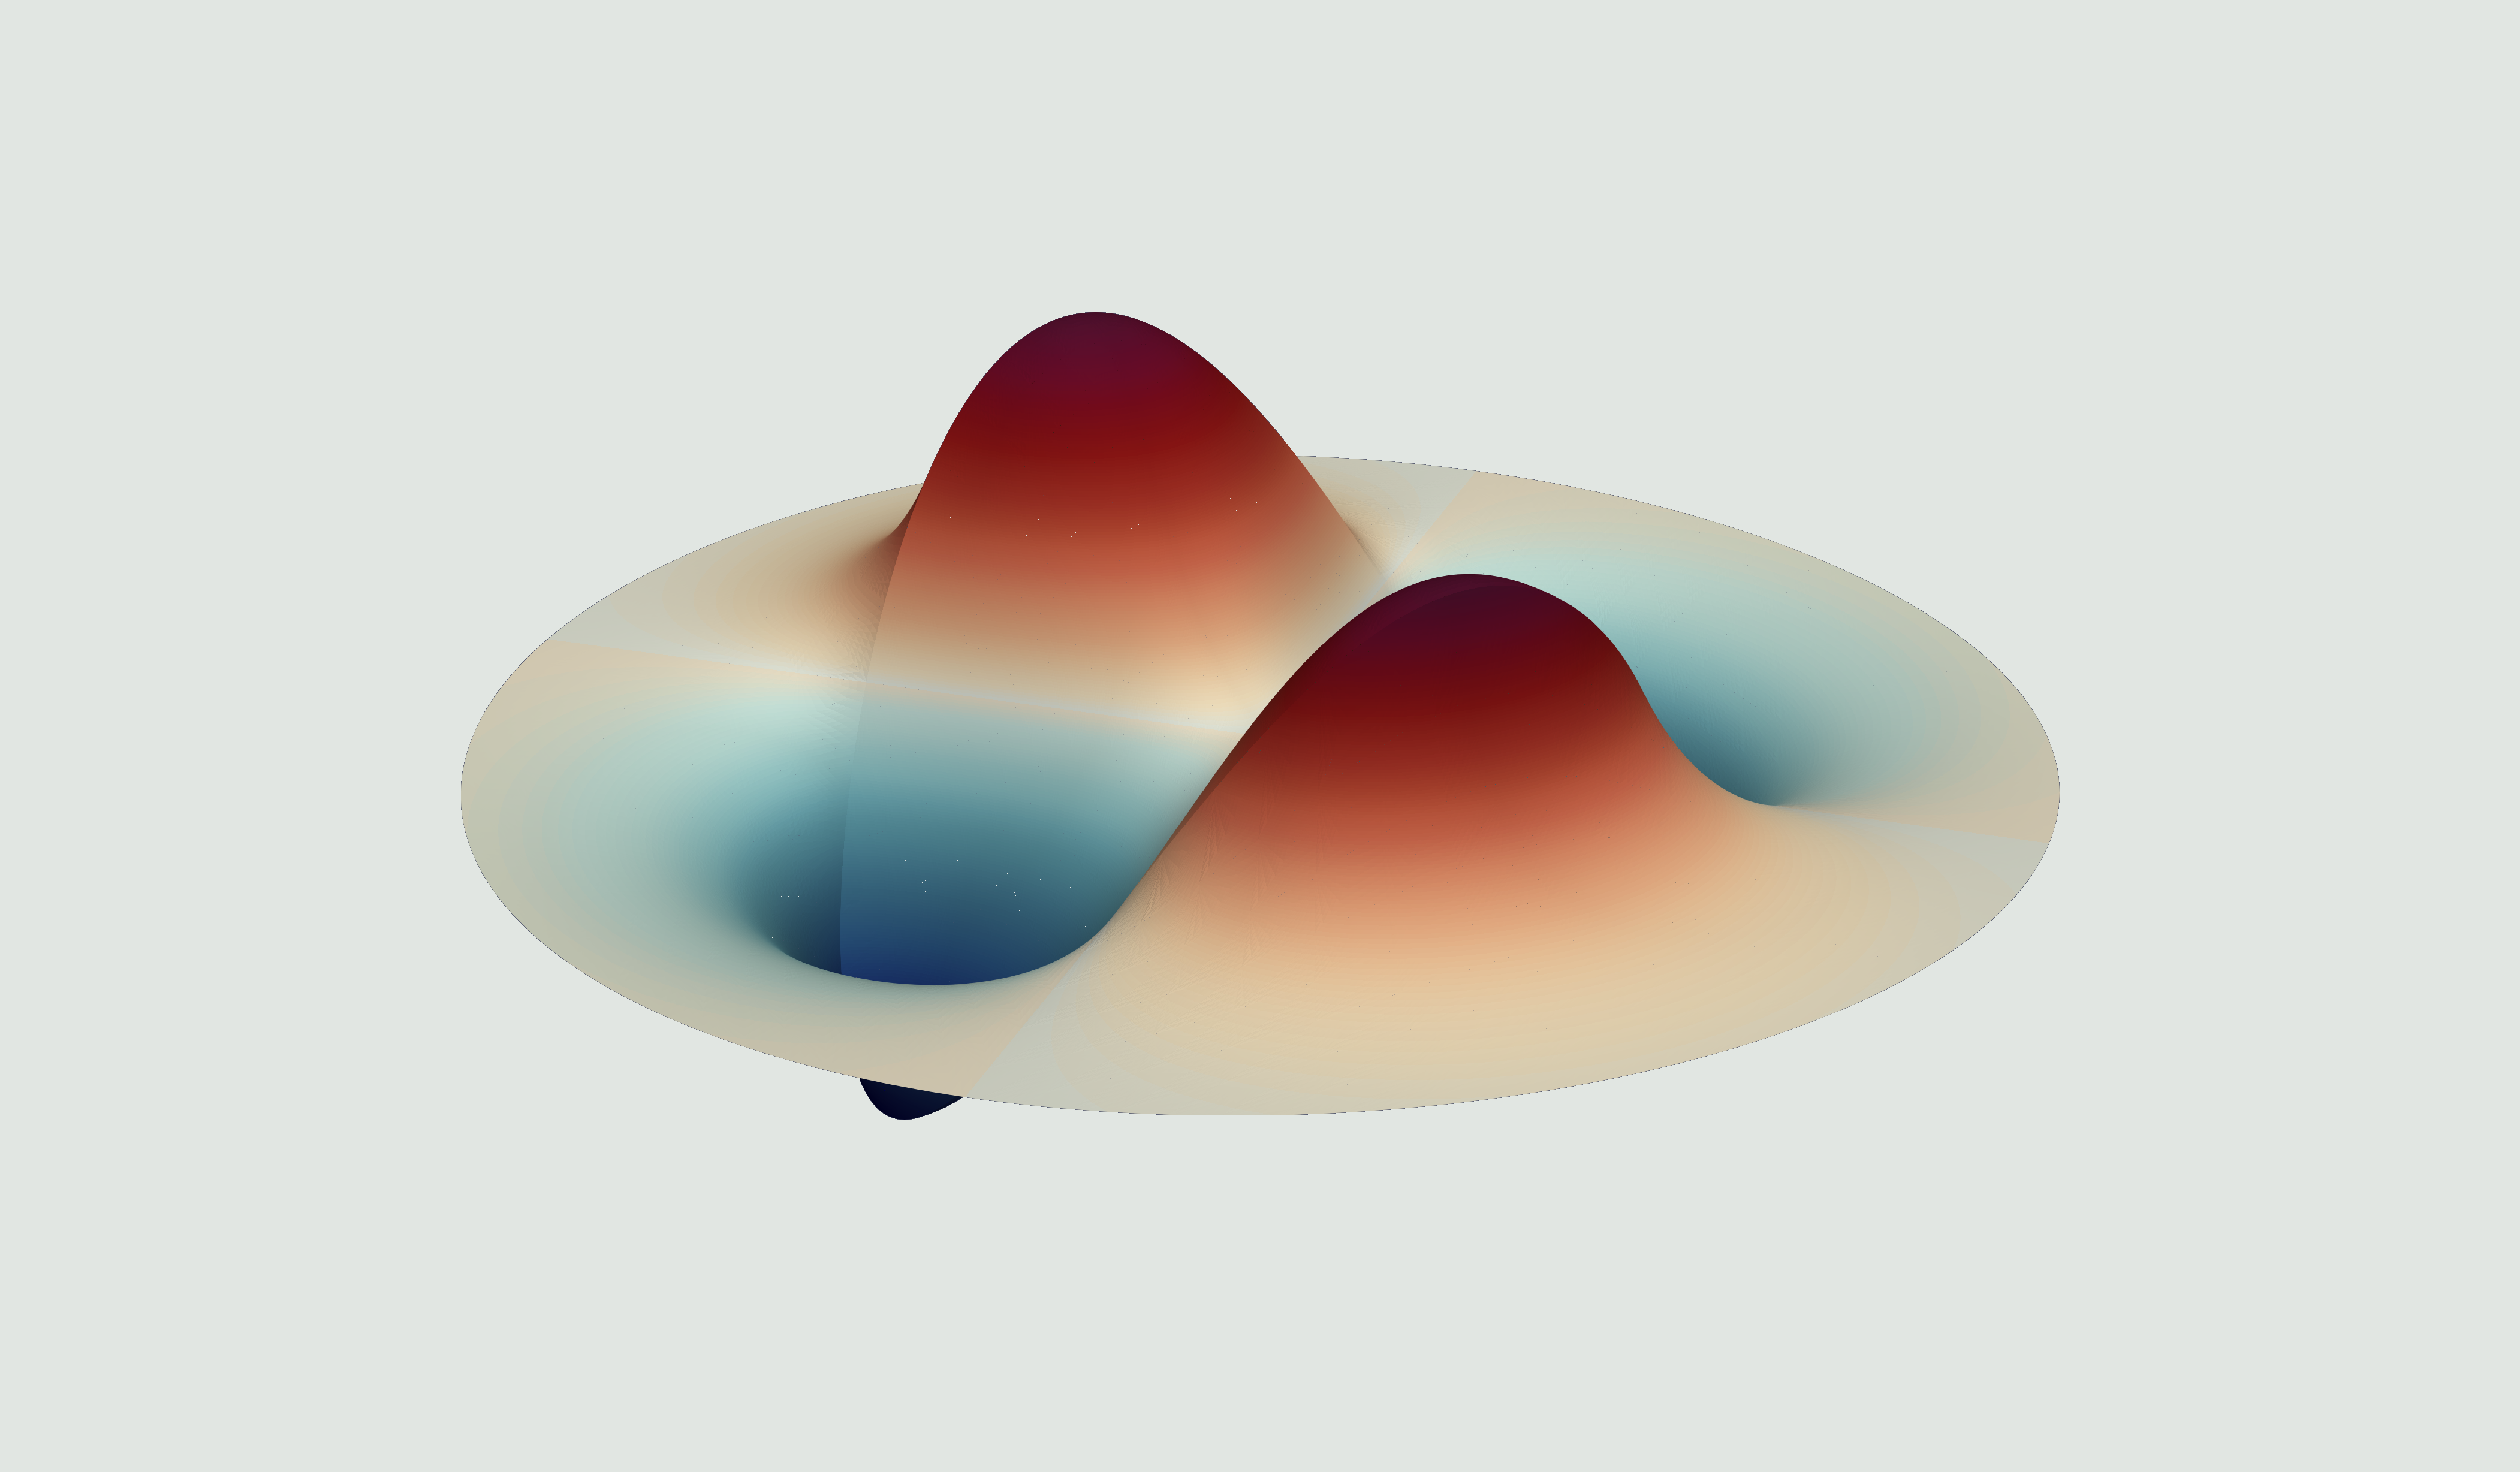
\includegraphics[width=1\linewidth]{images/ez3posterStepFiber.png}%
					\end{subfigure}
				\end{mdframed}
				\caption{The first two approximated LP modes for a step-index optical fiber with $r_{\text{\emph{core}}}=8\mu m$ and refractive indexes $n_1 =1.4457$(core) and $n_2 =1.4378$(cladding). The fiber is analyzed for $\lambda_0=1.55\mu m$. On the left, the Line Integral Convolution of the transversal component of the electric field is shown, and on the right its correspondent longitudinal component.}
				\label{fig:plot-step}
			\end{figure}
		\end{block}
    \end{minipage}\hspace{2cm}% <--- space
    \begin{minipage}[t]{0.45\textwidth}
        \begin{block}{\boxnumber HP-ADAPTIVITY CAPABILITIES }
        The developed basis functions, due to their hierarchical construction, can be easily integrated in the \emph{hp}-algorithms of the \texttt{NeoPZ} framework\parencite{diazcalle15}. In order to demonstrate its efficiency, the microstructured fiber presented in \parencite{chiang11} was analyzed. \Cref{fig:mesh-holey} shows a \emph{hp}-adaptive mesh in which the refinements were performed upon observation of the solution obtained with a fine mesh.
        \vspace*{1ex}

	        \begin{figure}
	        	\centering
		            \begin{tikzpicture}%
		        		\node[anchor=south west, inner sep=0] (X) at (0,0){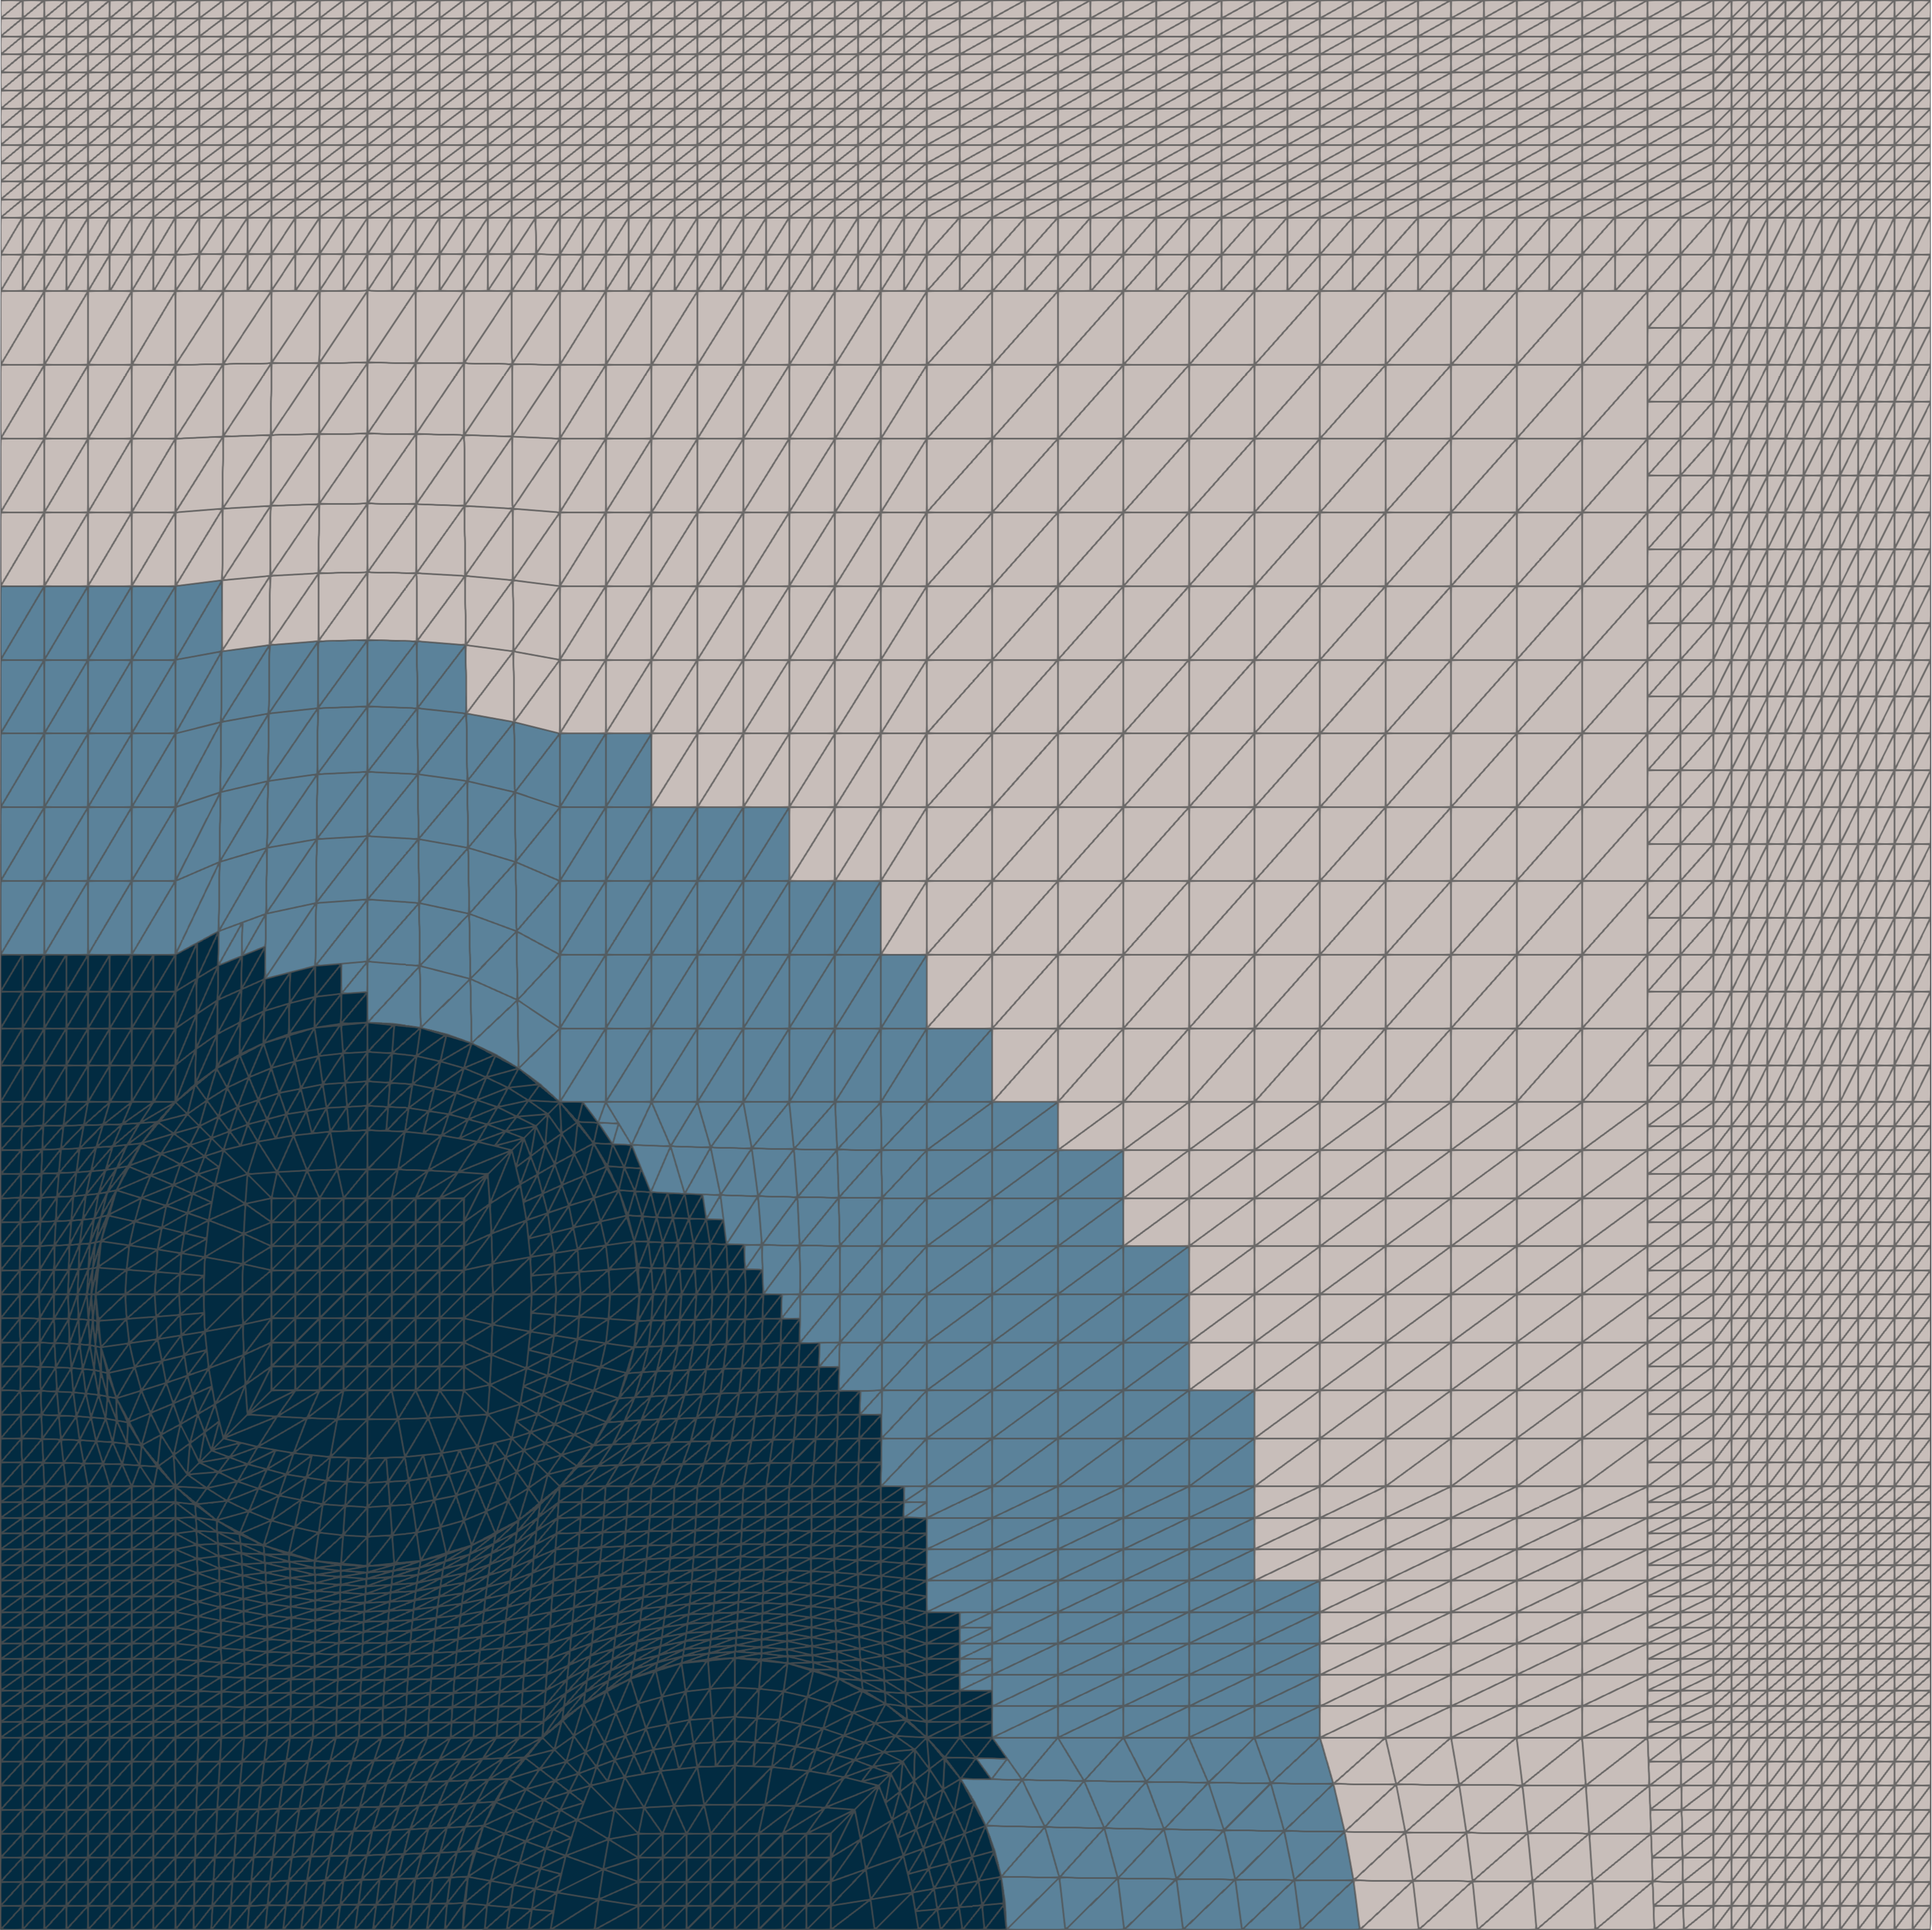
\includegraphics[height=0.8\linewidth]{images/holeyMesh.png}};%
		        		\begin{scope}[x={(X.south east)},y={(X.north west)}]%
		        		%% This makes all measurements with no units into fractions of the width
		        		%% and height of the graphic contained in the node.
		        		\draw[fill = white,fill opacity=0.8, text opacity=1] (0.05,0.075) rectangle (0.15,0.125) node[pos=.5] {$k=5$};
		        		\draw[fill = white,fill opacity=0.8, text opacity=1] (0.37,0.395) rectangle (0.47,0.445) node[pos=.5] {$k=4$};
		        		\draw[fill = white,fill opacity=0.8, text opacity=1] (0.65,0.675) rectangle (0.75,0.725) node[pos=.5] {$k=3$};
		        		\end{scope}%
		        		\node[anchor=south west, inner sep=0] (fig2) at (21,7.5){
\includegraphics[height=0.25\linewidth]{images/holeyMeshCrop.png}};%
		    	    \end{tikzpicture}
	    	    \caption{The Finite Element mesh of the microstructured fiber with six air-holes. The waveguide has a hole diameter of $d = 5\,\mu m$ and a hole pitch of $\Lambda=6.75\,\mu m$. The computational domain takes advantage of the symmetry of the desired fields and is a square with side $l=W+d_{pml}$, with $W=15.75\,\mu m$ and $d_{pml} = 2\, \mu m$. The elements have varying polynomial order from $k=3$ to $k=5$, and the mesh was refined on the region near the holes. The detail on the right highlights the presence of hanging nodes in the mesh.}
	    	    \label{fig:mesh-holey}
	    	\end{figure}    	
			\Cref{table:res-holey-conv} shows the significant reduction on the number of equations when using \emph{p} and \emph{hp}-refinement. While the number of equations is still higher than the ones obtained with the pseudospectral method in \textcite{chiang11}, the sparsity of the FEM matrices, allied with a solver that supports \emph{compressed row storage}(CRS) as \texttt{SLEPc}\parencite{slepc05} makes the FEM approach competitive in terms of memory and computational time. Finally, \Cref{fig:plot-holey} shows the electric field plots obtained with the mesh of \Cref{fig:mesh-holey}.

			\begin{table}[h]
				\caption{Effect of \emph{hp} mesh refinement on the number of equations and relative error of the approximated propagation constant in the microstructured fiber. In the example without refinement, $k=5$ was used for all elements. On the other two simulations, $3\leq k \leq 5$ was used, as shown in \Cref{fig:mesh-holey}.}
				\label{table:res-holey-conv}
				\begin{center}
					\begin{tabular}{lcc}
					 \toprule
					   & $n_{\text{\emph{eq}}}$    &    $e_{\text{\emph{rel}}}$   \\
					 \midrule
					 ---       & 285500 & $3.88420\times 10^{-13}$ \\
					 \emph{p}  & 181992 & $3.38410\times 10^{-13}$ \\
					 \emph{hp} & 130476 & $9.86280\times 10^{-13}$ \\
					 \bottomrule
					\end{tabular}
				\end{center}
			\end{table}

			\begin{figure}[hb]
	        	\begin{mdframed}[backgroundcolor=bggrey]
					\centering
					\begin{subfigure}[b]{.4999\textwidth}
						\centering
						\caption*{$\displaystyle\bm{E}_t$}
						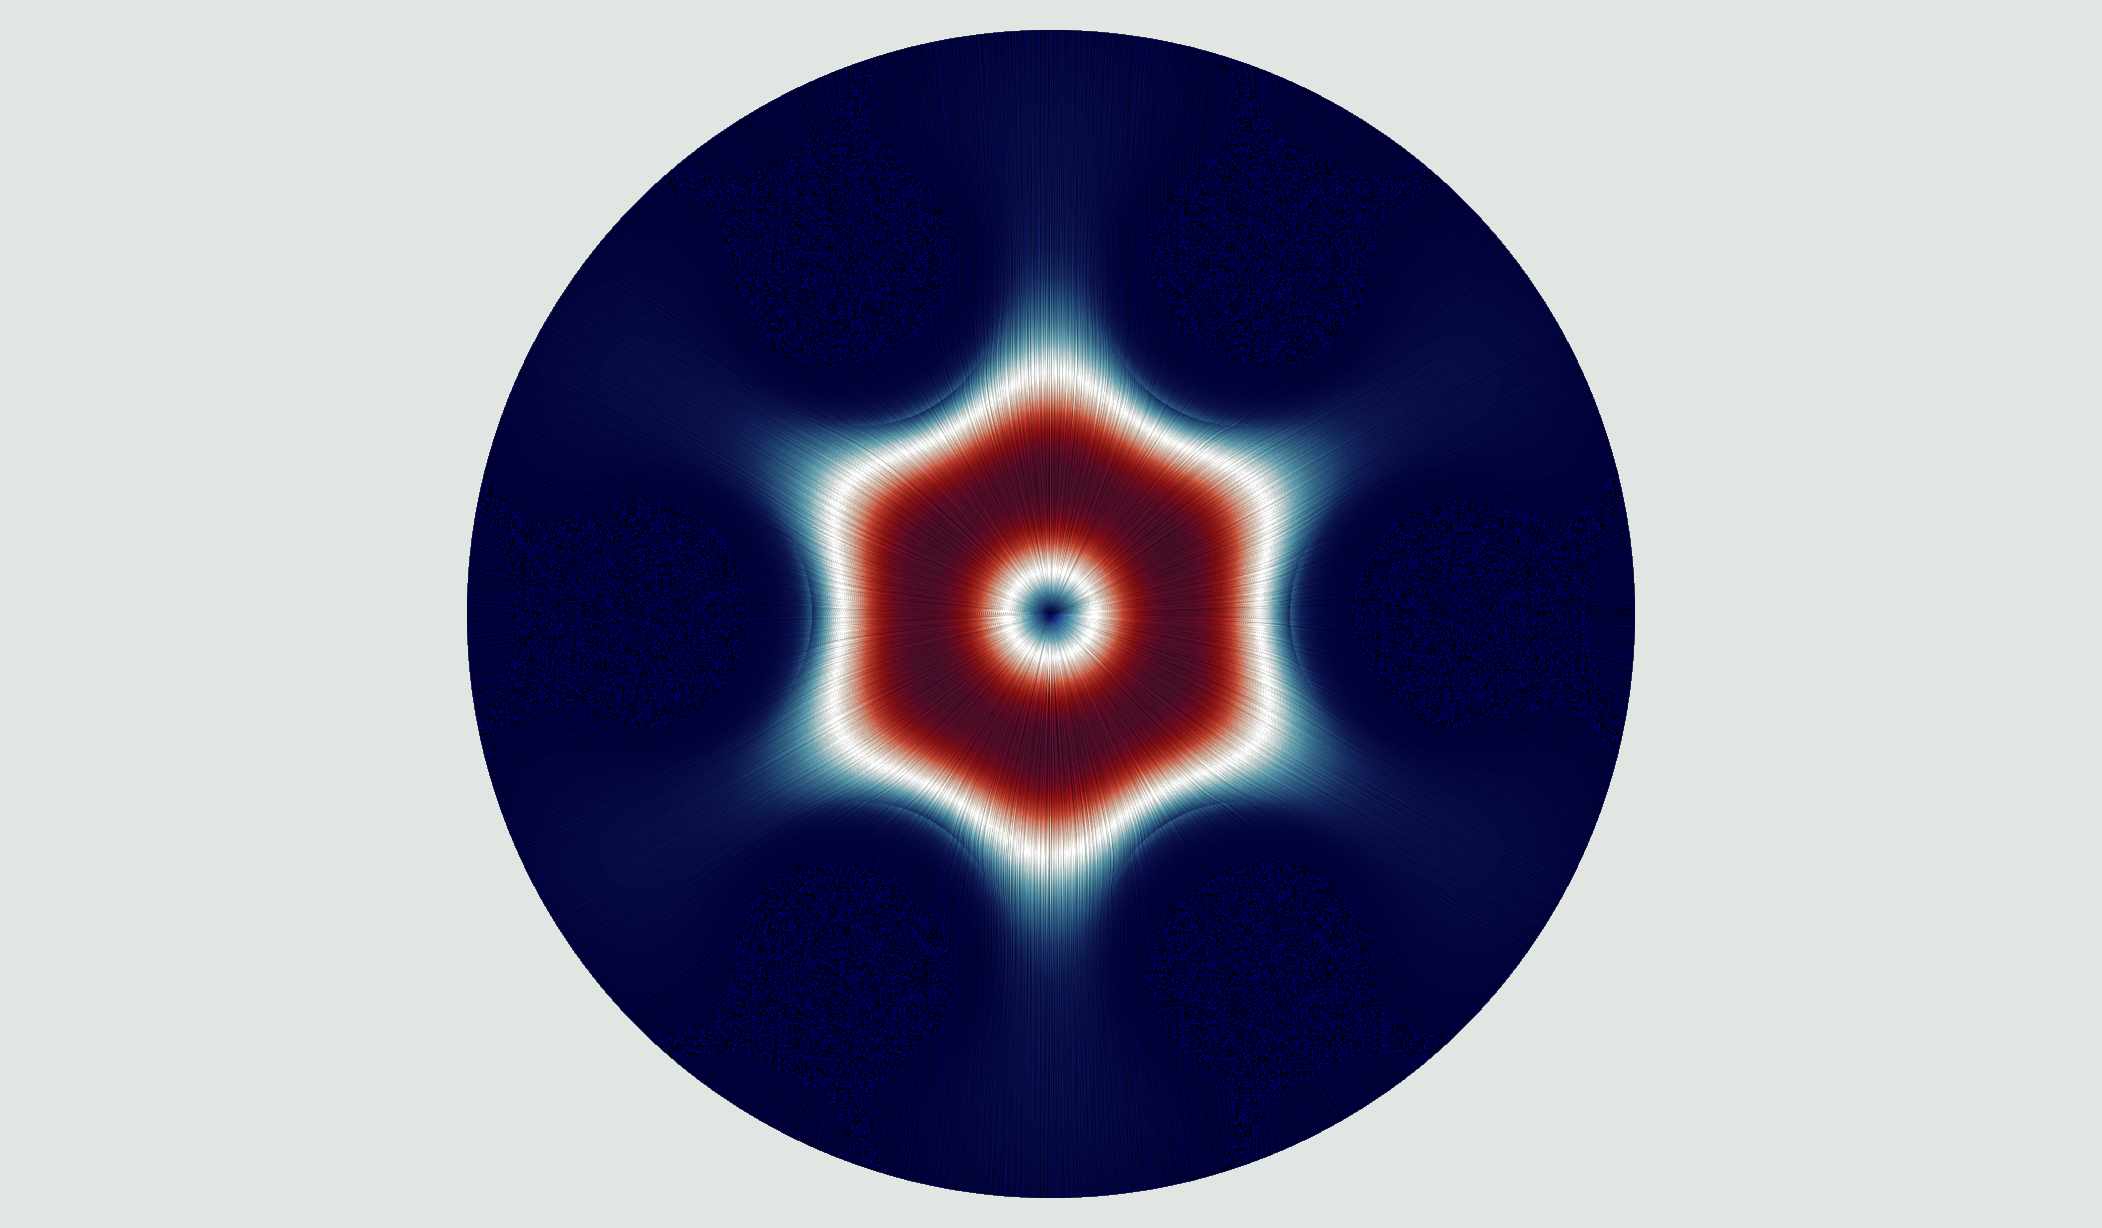
\includegraphics[width=1\linewidth]{images/et1posterHoley.png}%
					\end{subfigure}\hfill
					\begin{subfigure}[b]{.4999\textwidth}
						\centering
						\caption*{$\displaystyle E_z$}
						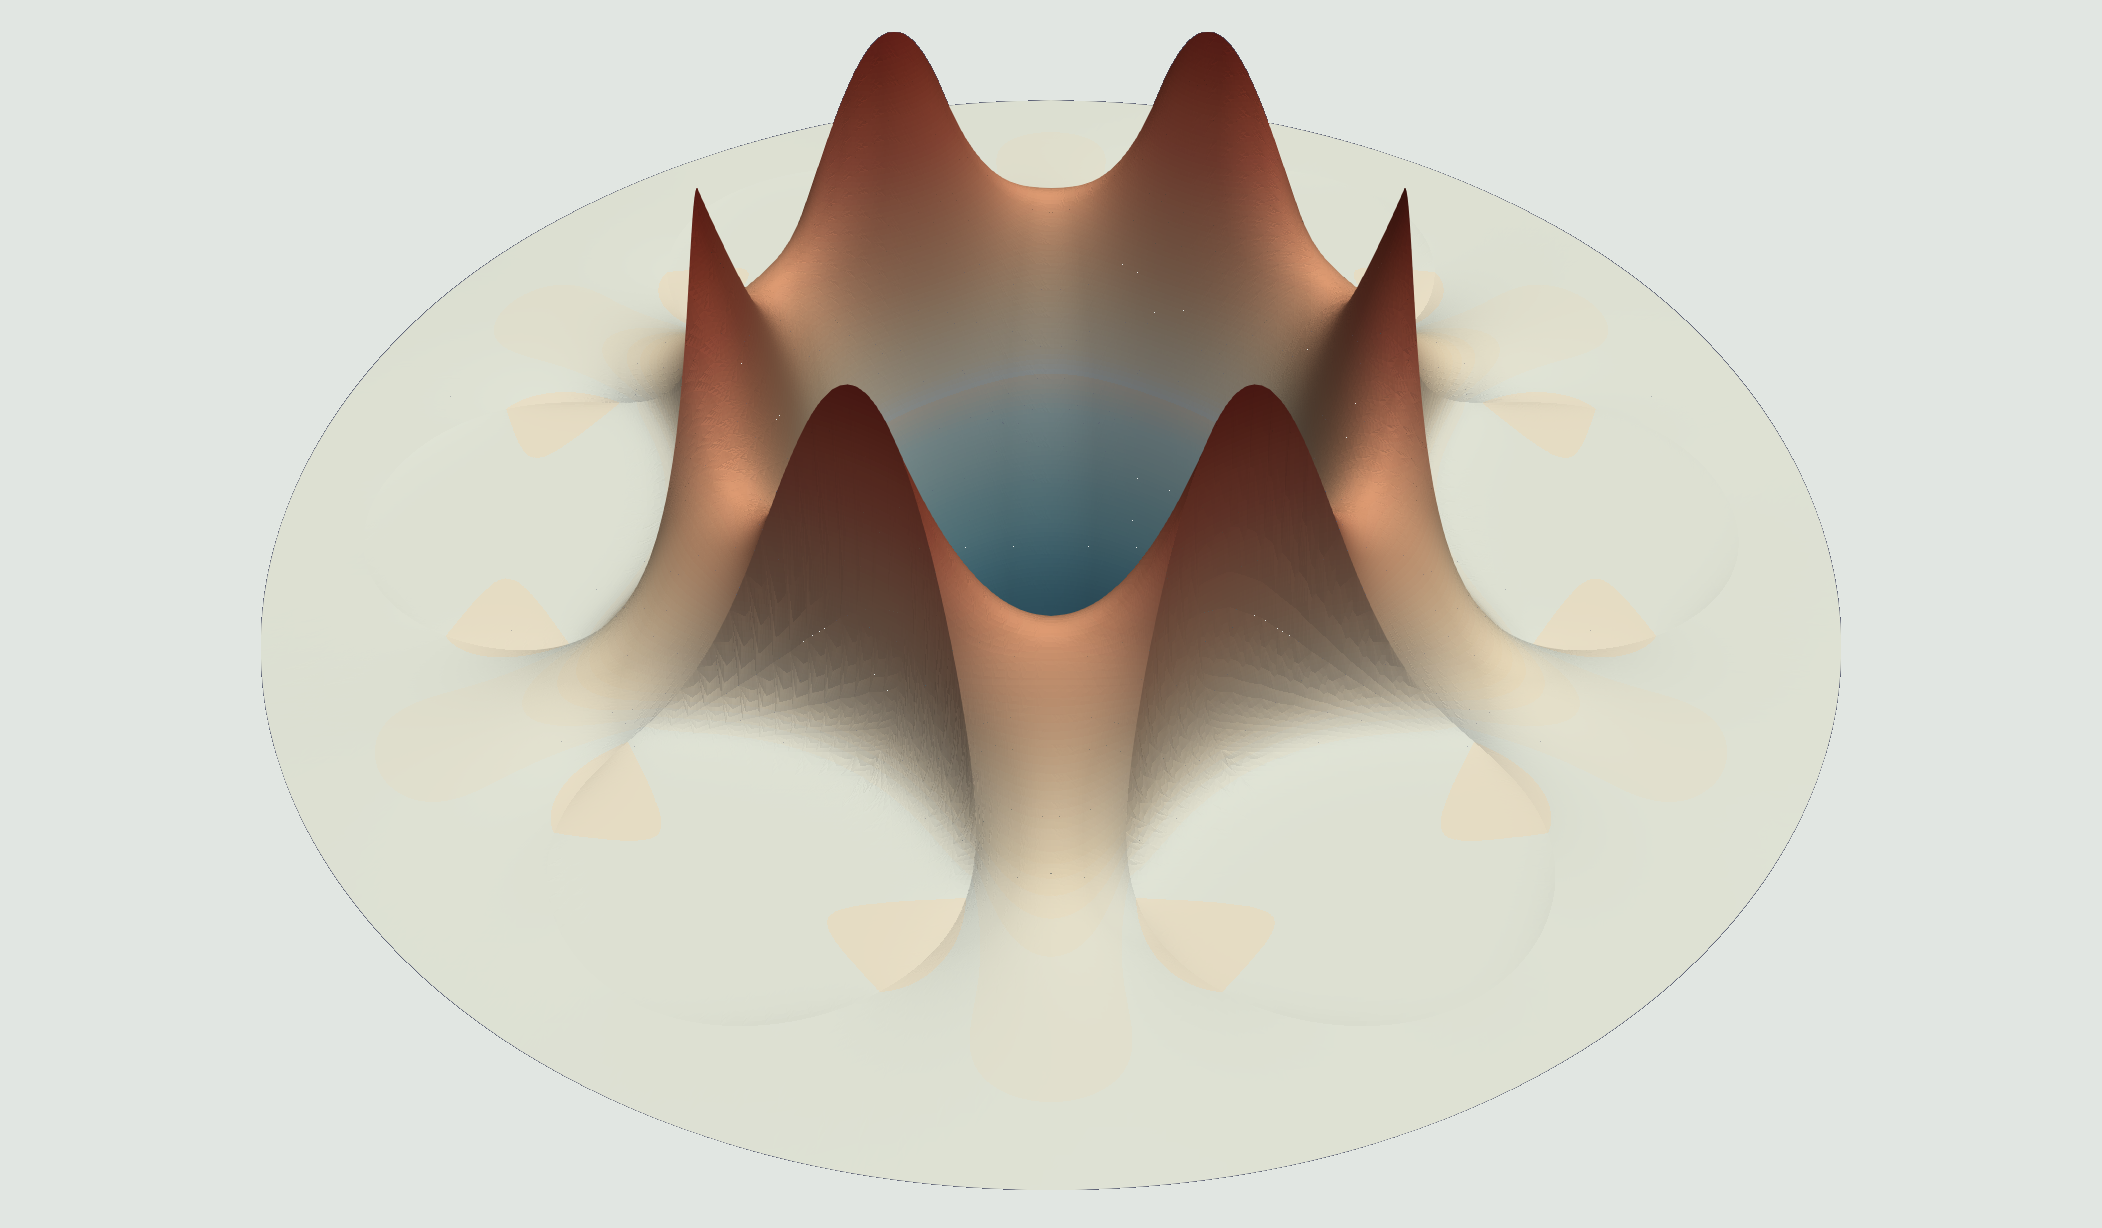
\includegraphics[width=1\linewidth]{images/ez1posterHoley.png}%
					\end{subfigure}

					\begin{subfigure}[b]{.4999\textwidth}
						\centering
						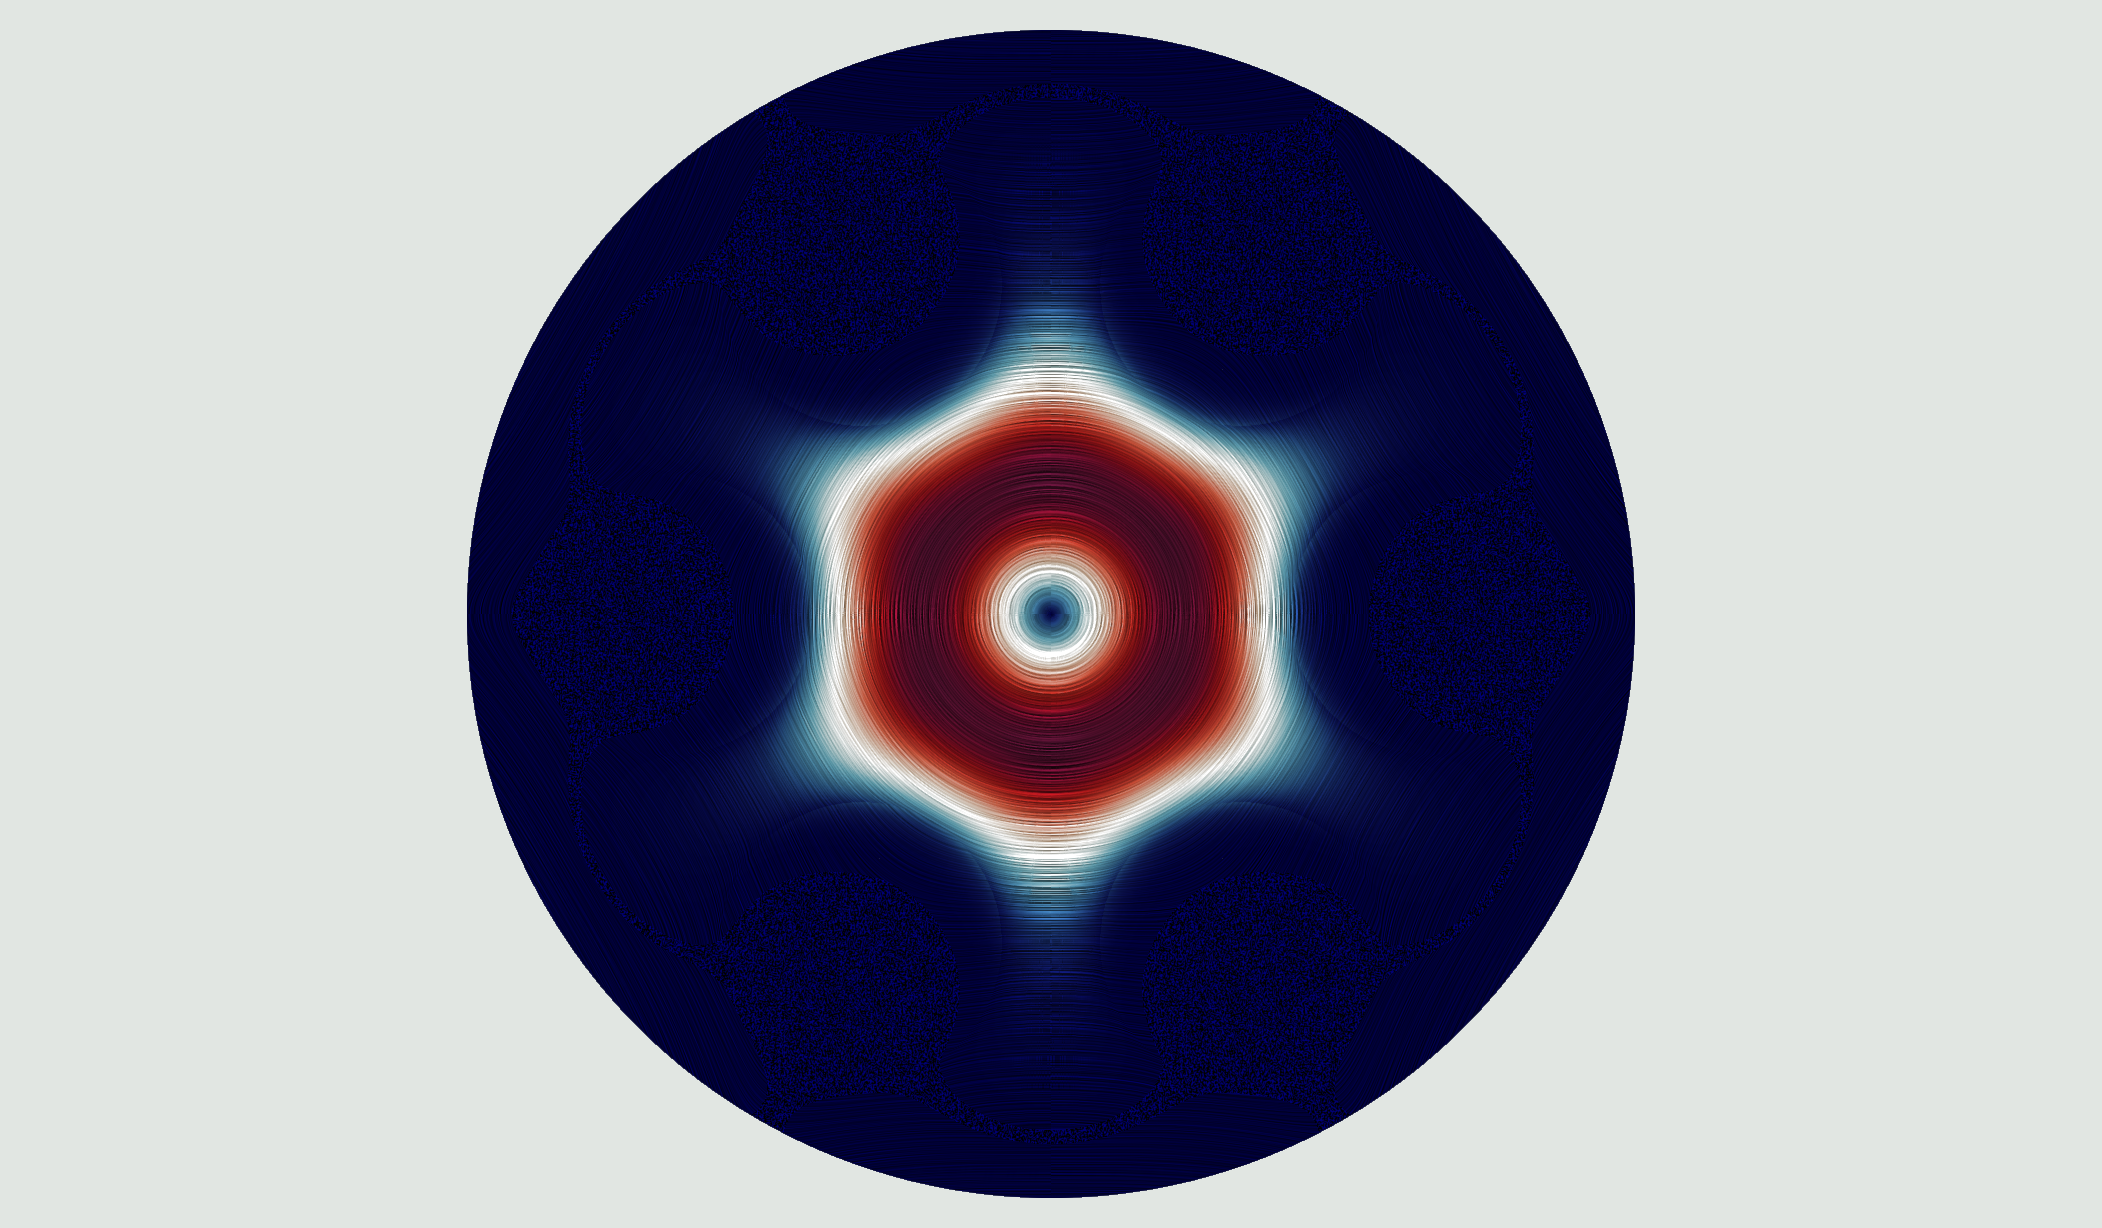
\includegraphics[width=1\linewidth]{images/et2posterHoley.png}%
					\end{subfigure}\hfill
					\begin{subfigure}[b]{.4999\textwidth}
						\centering
						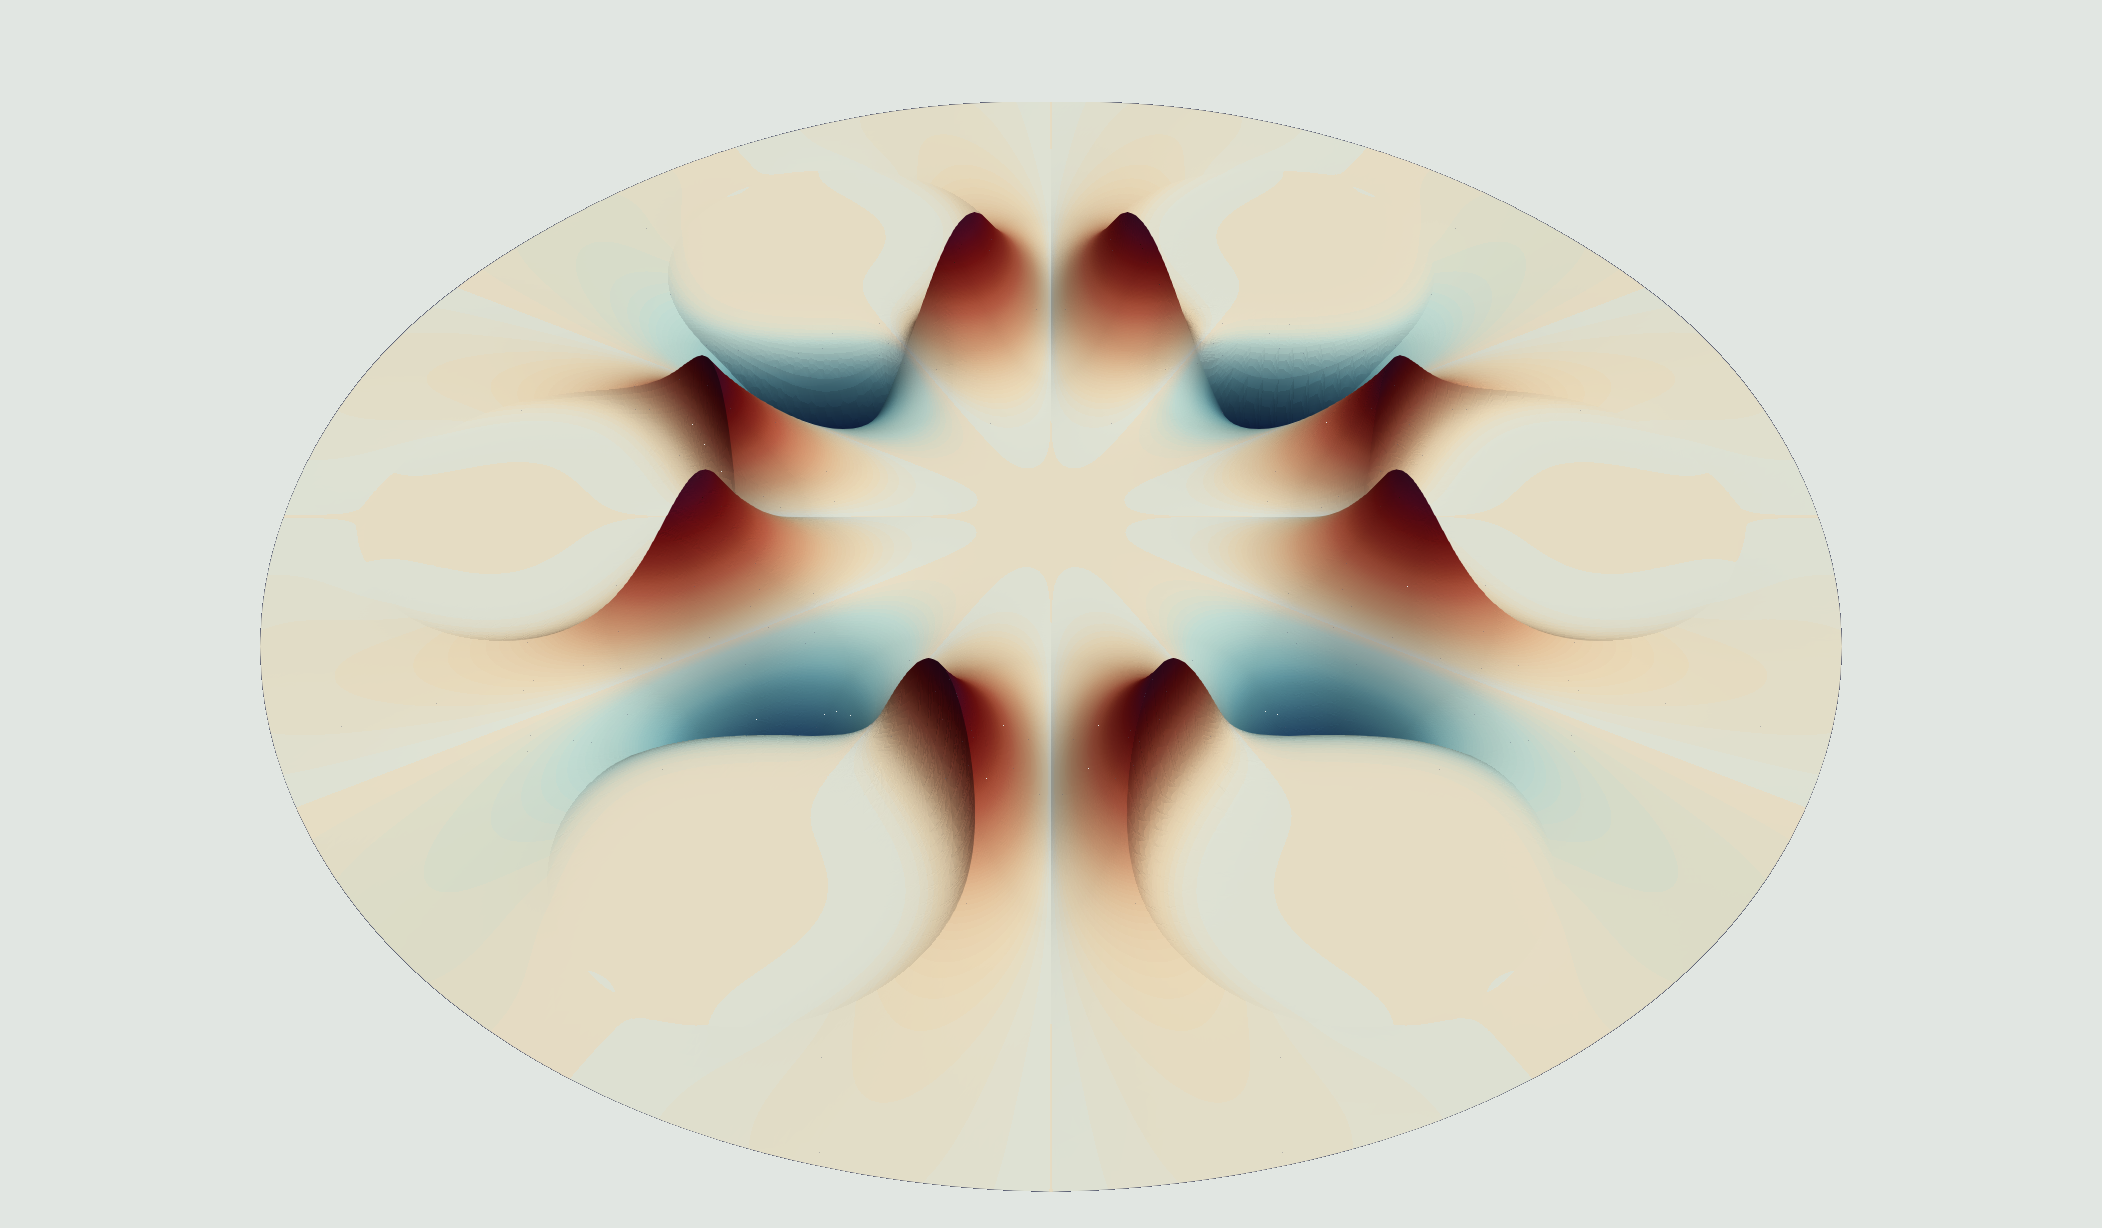
\includegraphics[width=1\linewidth]{images/ez2posterHoley.png}%
					\end{subfigure}
				\end{mdframed}
				\caption{Electric field plot of the sixth(up) and third(down) non-degenerated electromagnetic modes of the microstructured fiber. On the left, the Line Integral Convolution of the transversal component of the electric field is shown, and on the right its correspondent longitudinal component.}
				\label{fig:plot-holey}
			\end{figure}
        \end{block}
        \vfill
        \begin{block}{REFERENCES}
        	\printbibliography
        \end{block}
        %\vfill
    \end{minipage}
\end{frame}

\end{document}
